\begin{center}
	\color{blue!60!black}\textbf{BÀI TẬP OLYMPIC NGÀY 30/03}\\
	\textbf{PHẦN: NHIỆT HỌC}
\end{center}
% ===============================================================
\begin{ex}
	\immini{	Một mol khí lí tưởng đơn nguyên tử thực hiện một chu trình ABCDA được biểu diễn trên đồ thị $p-V$ có dạng hình bình hành như hình vẽ. Biết $p_\mathrm{A}=p_{\mathrm{B}}=3p_0$, $p_{\mathrm{C}}=p_{\mathrm{D}}=p_0$, $V_{\mathrm{A}}=V_0$, $V_{\mathrm{B}}=V_{\mathrm{D}}=7V_0$, trong đó $p_0$, $V_0$ coi như đã biết.
		\begin{enumerate}[label=\arabic*.]
			\item Tìm nhiệt độ lớn nhất và nhỏ nhất của khí trong chu trình trên.
			\item Tính hiệu suất của chu trình biết trung điểm M của đoạn BC chính là điểm chuyển đổi nhận nhiệt - tỏa nhiệt của khí trong quá trình BC.
	\end{enumerate}}
	{\begin{tikzpicture}  
			\begin{axis}[  ultra thick,scale=0.75,
				xmin=0,  
				xmax=15,  
				xtick={0,1,7},
				ytick={0,1,3},
				ymin=0,  
				ymax=4, 
				samples=300,
				yticklabels={0,$p_0$, $3p_0$},
				xticklabels={0,$V_0$, $7V_0$},
				axis lines=center, 
				xlabel=$V$, ylabel=$p$,
				every axis y label/.style={at=(current axis.above origin),anchor=south},  
				every axis x label/.style={at=(current axis.right of origin),anchor=west},  ]
				\coordinate (O) at (axis cs: 0,0);
				\coordinate (A) at (axis cs: 1,3);
				\coordinate (B) at (axis cs: 7,3);
				\coordinate (C) at (axis cs: 13,1);
				\coordinate (D) at (axis cs: 7,1);
				\draw[dashed, line width=1pt] (axis cs: 1,0)--(axis cs:1,3);
				\draw[dashed, line width=1pt] (axis cs:7,0)--(axis cs:7,1);
				\draw[dashed, line width=1pt] (axis cs:0,3)--(axis cs:7,3);
				\draw[dashed, line width=1pt] (axis cs:0,1)--(axis cs:7,1);
				\draw[blue, line width=1.5pt, decoration={markings, mark=at position 0.5 with {\arrow{stealth}}}, postaction={decorate}] (A)--(B);
				\draw[blue, line width=1.5pt, decoration={markings, mark=at position 0.75 with {\arrow{stealth}}}, postaction={decorate}] (B)--(C);
				\draw[blue, line width=1.5pt, decoration={markings, mark=at position 0.5 with {\arrow{stealth}}}, postaction={decorate}] (C)--(D);
				\draw[blue, line width=1.5pt, decoration={markings, mark=at position 0.5 with {\arrow{stealth}}}, postaction={decorate}] (D)--(A);
				\filldraw ($(B)!0.5!(C)$) circle(1pt);
			\end{axis}  
			\node[below left] at (O) {0};
			\node[above] at (A) {A};
			\node[above] at (B) {B};
			\node[right] at (C) {C};
			\node[right] at ($(B)!0.5!(C)+(0.2,0)$) {M};
			\node[below left] at (D) {D};
	\end{tikzpicture}}
	\hspace*{0pt}\hfill\textit{ĐS: 1. $T_{\max}=\dfrac{64p_0V_0}{3R}$, $T_{\min}=\dfrac{3p_0V_0}{R}$\quad 2. $H=\SI{23.4}{\percent}$.}
	
	\loigiai{
		
	}
\end{ex}
% ===============================================================
\begin{ex}
	Một bình cách nhiệt đựng nước đầy đến tận miệng ở nhiệt độ  $t_0=\SI{19}{\celsius}$. Người ta thả rất nhanh và nhẹ vào giữa bình một chi tiết máy làm bằng kim loại có khối lượng riêng $\rho_1=\SI{2700}{\kilogram/\meter^3}$ được nung nóng đến nhiệt độ $t_\mathrm{d}=\SI{99}{\celsius}$, và sau đó đóng chặt nắp bình. Sau khi có cân bằng nhiệt, nhiệt độ của nước trong bình $t_x=\SI{32.2}{\celsius}$. Sau đó, người ta đổ nước đầy từ đầu ở nhiệt độ $t_0=\SI{19}{\celsius}$, và lại thả nhanh và nhẹ hai chi tiết máy giống trên ở nhiệt độ $t_\mathrm{d}=\SI{99}{\celsius}$, và đóng nắp. Trong trường hợp này thì nhiệt độ cân bằng là $t_y=\SI{48.8}{\celsius}$. Nhiệt dung riêng $c_1$ của kim loại làm chi tiết trên bằng bao nhiêu? Khối lượng riêng của nước $\rho_0=\SI{1000}{\kilogram/\meter^3}$. Nhiệt dung riêng của nước $c_0=\SI{4200}{\joule/\left(\kilogram\cdot\kelvin\right)}$.\\
	\hspace*{0pt}\hfill\textit{ĐS: $c\approx\SI{920}{\joule/\left(\kilogram\cdot\kelvin\right)}$.}
	\loigiai{
		
	}
\end{ex}
% ===============================================================
\begin{ex} 
Súng phóc (ống thụt) là một thiết bị bắn đạn (thường là trái cò ke, quả đay, hoặc giấy ngâm nước cho mềm sau đó vo tròn thành viên, \dots) với tốc độ khá cao. Súng phóc bao gồm một ống tre hình trụ rỗng, một tay cầm có lắp  thanh trụ có chiều dài $L_0$  ngắn hơn chiều dài của ống tre $D$ và hai  viên đạn như hình bên dưới.
\begin{center}
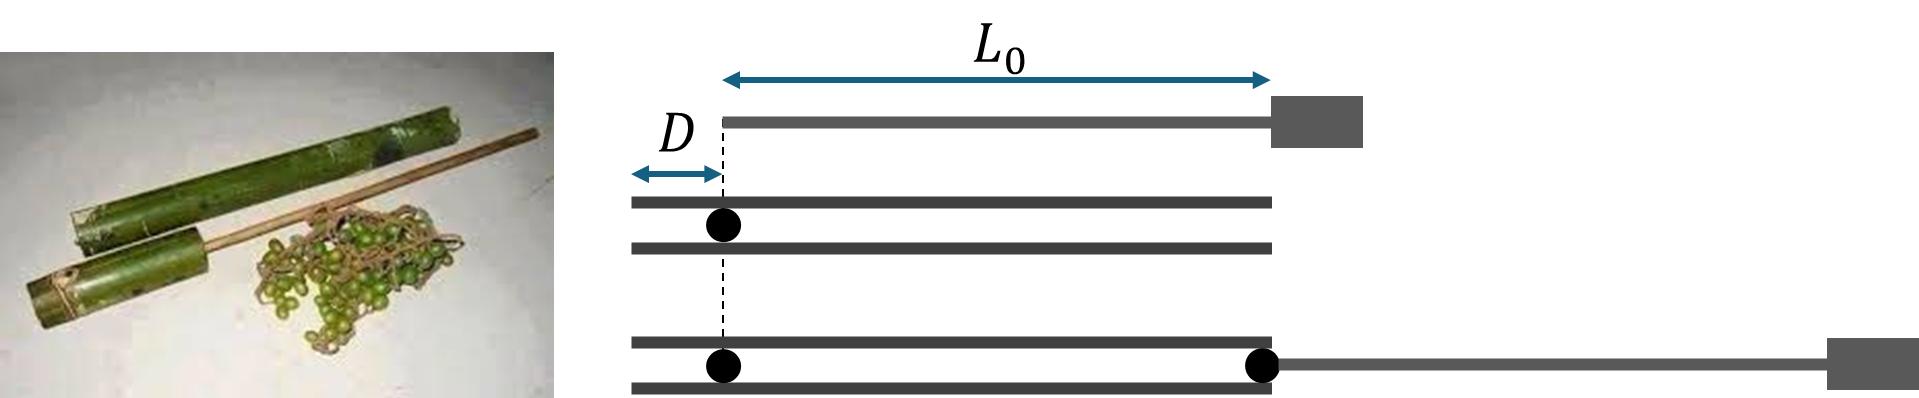
\includegraphics[scale=0.4]{figs/OLP-NHIET-01}
\end{center}
Viên đạn bên phải được thanh trụ của tay cầm đẩy đi dọc theo trục của ống tre, viên đạn bên trái bị giữ trong ống tre bởi lực ma sát nghỉ có giá trị lớn nhất là $F$. Đẩy nhanh viên đạn bên phải, khi khoảng cách giữa hai viên đạn đủ ngắn thì viên đạn bên trái bắt đầu chuyển động ra khỏi ống tre, lực ma sát giảm xuống là $f$ với $f\ll F$. Biết 
\begin{itemize}
	\item Mỗi viên đạn có khối lượng $m$, vừa khít với ống tre.
	\item Các viên đạn có đường kính rất nhỏ so với chiều dài $L_0$ và $D$.
	\item Tiết diện ngang phần rỗng của ống tre là $A$.
	\item Áp suất khí quyển là $p_\mathrm{A}$.
	\item Nhiệt dung mol đẳng tích $C_V$ và nhiệt dung mol đẳng áp $C_p$ không đổi.
\end{itemize}
\begin{enumerate}[label=\arabic*.]
	\item Quá trình nén không khí trong ống tre thuộc loại quá trình nhiệt động nào?
	\item Xác định khoảng cách giữa hai viên đạn khi viên đạn bên trái bắt đầu chuyển động.
	\item Xác định tốc độ ở cuối ống tre của viên đạn bên trái biết vận tốc của viên đạn bên trái lớn hơn rất nhiều so với vận tốc của thanh trụ.
	\item Xác định quãng đường $D$ để viên đạn có thể bắn ra với vận tốc lớn nhất.
\end{enumerate}

\hspace*{0pt}\hfill\textit{ĐS: 1. \smiley\quad 2. $L=L_0\left(\dfrac{p_0A}{F+p_0A}\right)^{\dfrac{1}{\gamma}}$.\quad 3. $v=\sqrt{\dfrac{2}{m}\left[\left(\dfrac{F+p_0A}{\gamma-1}\right)\left(L-L^\gamma\left(L+D\right)^{1-\gamma}\right)-\left(f+p_0A\right)D\right]}$.
}
 	\loigiai{
		
	}
\end{ex}
% ===============================================================
\begin{ex}
	Trong một bình hình trụ cách nhiệt có một piston và một cái van như hình. Van này mở ra và bắt đầu dẫn không khí từ bên ngoài vào trong bình khi chênh lệch áp suất là $\Delta p=\dfrac{p_0}{3}$ ($p_0$ là áp suất khí quyển), van không cho không khí ra khỏi bình. Ban đầu piston bị ép sát vào đáy bình, bên trong bình không có không khí. Hãy giải bài toán này trong 2 trường hợp như sau:
	\immini{\begin{enumerate}[label=\arabic*.]
			\item Bình được nạp đầy không khí đến thể tích $V_0$ bằng cách di chuyển piston một cách từ từ, sau đó dừng lại và thả piston ra. Xác định nhiệt độ không khí $T_1$ trong bình tại thời điểm piston dừng lại ở thể tích  $V_0$, cũng như nhiệt độ $T_2$ của không khí trong bình lúc piston dừng lại sau khi nó được thả ra.
			\item Piston chuyển đột ngột  đến vị trí mà thể tích không gian dưới piston có giá trị bằng $V_0$, vì piston chuyển động đột ngột  nên không khí không có thời gian đi qua van vào trong bình. Ở vị trí này, cố định piston, đợi cho đến khi bình chứa đầy không khí và giống như trường hợp đầu tiên, người ta thả piston ra.  Hãy xác định nhiệt độ không khí $T^\prime_1$ trong bình sau khi piston dừng lại và bình chứa đầy không khí, cũng như nhiệt độ $T^\prime_2$ của không khí trong bình khi piston dừng lại sau khi nó được thả ra để chuyển động. Giả sử rằng  quá trình nạp đầy không khí vào bình diễn ra gần như tĩnh, van đóng lại ngay lập tức sau khi chênh lệch áp suất nhỏ hơn ngưỡng. Bên ngoài bình có không khí ở áp suất $p_0$ và nhiệt độ $T_0$.\\	\end{enumerate}}
{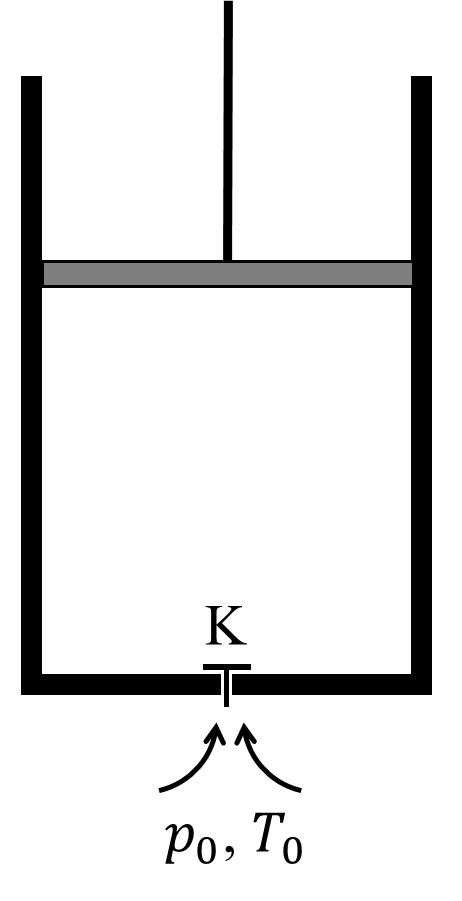
\includegraphics[scale=0.4]{figs/OLP-NHIET-02}}
	Có thể bỏ qua ma sát giữa piston và thành bình, khối lượng piston, sự trao đổi nhiệt của không khí với piston và thành bình. Không khí có thể được coi là khí lí tưởng lưỡng nguyên tử. Sau khi thả piston thì van luôn đóng.\\
	\hspace*{0pt}\hfill\textit{ĐS: 1. $T_1=T_0$, $T_2=\dfrac{8T_0}{7}$ \quad 2. $T^\prime_1=\dfrac{7T_0}{5}$, $T^\prime_2=\dfrac{8T_0}{5}$.}
	\loigiai{
		
	}
\end{ex}
\begin{center}
	\textbf{--- HẾT ---}
\end{center}
